%%%%%%%%%%%%%%%%%%%%%%%%%%%%%%%%%%%%%%%%%%%%%%%
%%%     Declarations (skip to Begin Document, line 88, for parts you fill in)
%%%%%%%%%%%%%%%%%%%%%%%%%%%%%%%%%%%%%%%%%%%%%%%

%%\documentclass[10pt]{article}
%%\documentclass[10pt]{report}
\documentclass[letterpaper]{article}
\usepackage{geometry}
%\usepackage{xcolor}
\usepackage[table]{xcolor}
\usepackage{amsmath}
\usepackage[some]{background}
%\usepackage{lipsum}
%\usepackage{natbib}
\usepackage[utf8]{inputenc} % set input encoding to utf8

 
% C I T A T I O N S
%\usepackage[backend=biber,style=apa]{biblatex}
\usepackage[backend=biber, bibstyle=numeric, citestyle=numeric]{biblatex} 
\DeclareLanguageMapping{english}{english-apa}
%\usepackage{apacite}
%\bibliographystyle{apa}

%\usepackage{biblatex} 
\addbibresource{paperpile.bib}
\usepackage{datetime}

%\usepackage{hyperref}

% Tables
\usepackage{float}
\usepackage[utf8]{inputenc}
\usepackage{tabularx}
\usepackage{booktabs}
\usepackage{longtable}

\usepackage{diagbox} %table split headers
\usepackage{longtable}
\usepackage{array}
\usepackage{rotating}
\usepackage{eqparbox}
\usepackage{makecell, caption, booktabs}
\usepackage{tablefootnote}

\usepackage{colortbl}

% Stuff needed to get table to span pages
\usepackage{enumitem}
%\usepackage{array, booktabs, longtable}
\newcolumntype{x}[1]{>{\raggedright}p{#1}}

\usepackage{etoolbox}
\AtBeginEnvironment{longtable}{%
    \setlist[itemize]{nosep,     % <-- new list setup
                      topsep     = 0pt       ,
                      partopsep  = 0pt       ,
                      leftmargin = *         ,
                      label      = $\bullet$ ,
                      before     = \vspace{-\baselineskip},
                      after      = \vspace{-0.5\baselineskip}
                        }
                           }% end of AtBeginEnvironment
% End table span

\definecolor{green}{rgb}{0.1,0.1,0.1}
%\color{green!40!yellow})

\newcommand{\done}{\cellcolor{teal}done}  %{0.9}
\newcommand{\hcyan}[1]{{\color{teal} #1}}

% Listings
\usepackage{listings}

\usepackage{geometry}  % Lots of layout options.  See http://en.wikibooks.org/wiki/LaTeX/Page_Layout
\geometry{letterpaper}  % ... or a4paper or a5paper or ... 
\usepackage{fullpage}  % somewhat standardized smaller margins (around an inch)
\usepackage{setspace}  % control line spacing in latex documents
\usepackage[parfill]{parskip}  % Activate to begin paragraphs with an empty line rather than an indent

\usepackage{amsmath,amssymb}  % latex math
\usepackage{empheq} % http://www.ctan.org/pkg/empheq
\usepackage{bm,upgreek}  % allows you to write bold greek letters (upper & lower case)

% for typsetting algorithm pseudocode see http://en.wikibooks.org/wiki/LaTeX/Algorithms_and_Pseudocode
\usepackage{algorithmic,algorithm}  

\usepackage{graphicx}  % inclusion of graphics; see: http://en.wikibooks.org/wiki/LaTeX/Importing_Graphics
% allow easy inclusion of .tif, .png graphics
\DeclareGraphicsRule{.tif}{png}{.png}{`convert #1 `dirname #1`/`basename #1 .tif`.png}

% \usepackage{subfigure}  % allows subfigures in figure
\usepackage{caption}
\usepackage{subcaption}

\usepackage{xspace}
\newcommand{\latex}{\LaTeX\xspace}

\usepackage{color}  % http://en.wikibooks.org/wiki/LaTeX/Colors

\long\def\todo#1{{\color{red}{\bf TODO: #1}}}

\long\def\ans#1{{\color{blue}{\em #1}}}
\long\def\ansnem#1{{\color{blue}#1}}
\long\def\boldred#1{{\color{red}{\bf #1}}}
\long\def\boldred#1{\textcolor{red}{\bf #1}}
\long\def\boldblue#1{\textcolor{blue}{\bf #1}}

% Useful package for syntax highlighting of specific code (such as python) -- see below
\usepackage{listings}  % http://en.wikibooks.org/wiki/LaTeX/Packages/Listings
\usepackage{textcomp}


%%% The following lines set up using the listings package
\renewcommand{\lstlistlistingname}{Code Listings}
\renewcommand{\lstlistingname}{Code Listing}

%%% Specific for python listings
\definecolor{gray}{gray}{0.5}
\definecolor{green}{rgb}{0,0.5,0}

\lstnewenvironment{python}[1][]{
\lstset{
language=python,
basicstyle=\footnotesize,  % could also use this -- a little larger \ttfamily\small\setstretch{1},
stringstyle=\color{red},
showstringspaces=false,
alsoletter={1234567890},
otherkeywords={\ , \}, \{},
keywordstyle=\color{blue},
emph={access,and,break,class,continue,def,del,elif ,else,%
except,exec,finally,for,from,global,if,import,in,i s,%
lambda,not,or,pass,print,raise,return,try,while},
emphstyle=\color{black}\bfseries,
emph={[2]True, False, None, self},
emphstyle=[2]\color{green},
emph={[3]from, import, as},
emphstyle=[3]\color{blue},
upquote=true,
morecomment=[s]{"""}{"""},
commentstyle=\color{gray}\slshape,
emph={[4]1, 2, 3, 4, 5, 6, 7, 8, 9, 0},
emphstyle=[4]\color{blue},
literate=*{:}{{\textcolor{blue}:}}{1}%
{=}{{\textcolor{blue}=}}{1}%
{-}{{\textcolor{blue}-}}{1}%
{+}{{\textcolor{blue}+}}{1}%
{*}{{\textcolor{blue}*}}{1}%
{!}{{\textcolor{blue}!}}{1}%
{(}{{\textcolor{blue}(}}{1}%
{)}{{\textcolor{blue})}}{1}%
{[}{{\textcolor{blue}[}}{1}%
{]}{{\textcolor{blue}]}}{1}%
{<}{{\textcolor{blue}<}}{1}%
{>}{{\textcolor{blue}>}}{1},%
%framexleftmargin=1mm, framextopmargin=1mm, frame=shadowbox, rulesepcolor=\color{blue},#1
framexleftmargin=1mm, framextopmargin=1mm, frame=single,#1
}}{}
%%% End python code listing definitions

\DeclareMathOperator{\diag}{diag}
\DeclareMathOperator{\cov}{cov}


%\bibliography{./paperpile.bib}
\author{Evan McGinnis}
\title{Automated Weeding}



\definecolor{titlepagecolor}{cmyk}{1,.60,0,.40}

\DeclareFixedFont{\bigsf}{T1}{phv}{b}{n}{1.5cm}

\backgroundsetup{
scale=1,
angle=0,
opacity=1,
contents={\begin{tikzpicture}[remember picture,overlay]
 \path [fill=titlepagecolor] (-0.5\paperwidth,5) rectangle (0.5\paperwidth,10);  
\end{tikzpicture}}
}
\makeatletter                       
\def\printauthor{%                  
    {\large \@author}}              
\makeatother
\author{%
    Evan McGinnis \\
    PhD Student \\
    Student ID\#  23633780\\
    Biosystems Analytics \\
    \today \\
    \texttt{evanmc@email.arizona.edu}\vspace{40pt} \\
    }

\begin{document}

\begin{titlepage}
\BgThispage
\newgeometry{left=1cm,right=4cm}
\vspace*{1cm}
\noindent
%%\vspace*{0.4\textheight}
\textcolor{white}{\Huge\textbf{\textsf{A Proposal for Automated Weeding\\ in Lettuce Crop}}}
\vspace*{2.5cm}\par
\noindent
\begin{minipage}{0.35\linewidth}
    \begin{flushright}
        \printauthor
    \end{flushright}
\end{minipage} \hspace{15pt}
%
\begin{minipage}{0.02\linewidth}
    \rule{1pt}{175pt}
\end{minipage} \hspace{-10pt}
%
\begin{minipage}{0.6\linewidth}
\vspace{5pt}
    \begin{abstract} 
This paper proposes a study of a automated weeding system for lettuce cultivars.  The system consists of three major subsystems, image processing,  control, and treatment. Of these three subsystems, the image processing and control systems are the subject of this study. The image processing system uses machine learning to distinguish weed from crop and will direct treatment of vegetation deemed to be a weed.
    \end{abstract}
\end{minipage}
\end{titlepage}
\restoregeometry
%
% F R O N T  M A T T E R
%
\tableofcontents
\listoffigures
\newpage

%
% B E G I N   T E M P L A T E   F R O M   W O R D
%

%
% O V E R V I E W
%

\section{Overview}
%This paper proposes a study of an automated weeding system for lettuce cultivars.  The automated weeding system will be proven at the Yuma agricultural center, and the conditions explored in this study (economic, field) will be used to reflect specific examples. 
%There are two motivations for the exploration of automation for this use case: health of agricultural workers, and economics of manual labor. The link between exposure to synthetic herbicides and negative impacts on agricultural workers has been long been well established, and a direct impact of this proposal is to minimize that exposure. Personal protective equipment (PPE) is sometimes cited as a solution to minimizing exposure, but is more often adopted during the mixing phase of chemicals than it is during the application (\cite{Macfarlane2008-am}). Economically, the case for an automation solution involves two aspects: the availability of labor, and once found, the overall cost of that labor. There is little doubt that manual weeding is a tedious, difficult task. Even when recruited for, the costs for this labor put pressure on profit margins associated with the crop.  In Yuma, AZ, for example, the labor cost for manual weeding of an acre of lettuce often exceeds \$100 \cite{Siemens2021-vn} and the mean hourly wage is \$14.78 per hour per worker \cite{US_Bureau_of_Labor_Statistics2021-yi}.

\label{section:proposal}
This study will produce a commercially viable, tractor-mounted, automated weeding system for lettuce cultivars. The proposed system will obviate the need for manual weed remediation, and use two technologies to achieve this: machine learning and precision spraying. \textit{Commercially viable} has two dimensions that are key to the success of this proposal: accuracy and speed. The automation achieved by the system must be both highly accurate (above 95\%) and performed quickly enough that a system can perform the task of weed control at acceptable speeds (around 200 ms per image to support a tractor speed of 4kph). 

\section{Introduction}
Manual weed control by mechanical means in row crops is expensive, and labor willing to perform this field work is increasingly hard to find. Alternatively, weed control using manual chemical application is not only expensive, but is a harm to both the environment and worker's health. 
This work will yield an automated system that will lower costs and decrease threats to both worker health and the environment, all while achieving high treatment accuracy.  By integrating precision sprayers with new work in machine vision, weed/crop discrimination, and networked system design, this proposal will achieve these goals.\footnote{The mechanical components (enclosure as the electrical and pneumatic systems that support the precision sprayer) used in a field deployment and towed behind a tractor are already developed, and will not be addressed in depth by this proposal.}
This study will use morphological and color features to distinguish between crop and weeds, and weeds will be the target of subsequent treatment. There are three activities that warrant attention here: separation of vegetation from background, feature extraction, and weed/crop discrimination,\\
Aspects of this problem are well researched in documented. Hamuda surveys the task of separation of vegetation and non-vegetated portions of visible light images, and that work will be used in this proposal \parencite{Hamuda2016-dw}. The disadvantages mentioned of color-index based schemes (changing lighting conditions lead to inconsistent results, and the expected dominant color of vegetation is green) will not be of concern for this work, as the lighting will be controlled (it will be artificial) and both crop and weeds will be predominately green.\\
There are two types of features to be considered: color and structural. Sabzi studies both of these feature types in a study of weed identification \parencite{Sabzi2020-af}. Color feature evaluation was carried out in \textit{transformed} color spaces: Hue, Saturation, Intensity (HSI); Hue, Saturation, Value (HSV); Luminance, In-Phase, Quadrature (YIQ); and Luminance, blue - luminance, and red - luminance (YCbCr). Structural features were not heavily emphasized in this model, as the area-to-length ratio was the sole structural component considered. While the correct classification rate in that study exceeded 98\%, the field tests showed a commercially nonviable speed of 0.15 m/s. \\
Lin, in a study of corn and weed species identification, identifies key shape features, along with formulae for their determination that can then be exploited in discrimination: shape index and length-to-width ratio \parencite{Lin2017-xq}. Wirth, in a presentation on shape analysis, details aspects of (and formulae for) structural features of objects. Among these are: roundness, convexity, solidity, elongation, and compactness \parencite{Wirth2004-li}.\\
Using both color and morphological features it is possible to achieve both the speed and accuracy required in weed identification. While research has shown that distinguishing crop from weeds is possible given sufficient computing resources, doing so in a field setting with limited computational power is not fully addressed. Coupling an image recognition system to a treatment system is often left as a exercise for the reader or mentioned as a possible application. This study will provide a complete solution.


\subsection{Results}
Analysis of a set of visible-light images\footnote{Image set of lettuce beds supplied by Dr. Mark Siemens} shows that various approaches were used in classifying the objects isolated in the images and detailed in Table~\ref{fig:learning}.

{\renewcommand{\arraystretch}{2}%
\begin{table}[H]
	\centering
    	\caption{Machine Learning Results}
   	 \label{fig:learning}
   	 \begin{tabular}{  l  p{4cm}  p{5cm} }
        	\toprule
		\textbf{Method}      
		& \textbf{Train}   
		& \textbf{Test} \\\midrule
		Logistic Regression
		& 0.9790       
		& 0.9787 \\\hline
		KNN     
		& $1.0$                    
		& $0.86$ \\\hline
		Decision Tree
		& 1.0
		& 0.96 \\\hline
		Boosted Gradient     
		& 1.0
		& 0.957 \\\hline
		Random Forest      
		& 1.0
		& 0.986 \\\hline
       	 \bottomrule
	\end{tabular}
\end{table}

\subsection{Discussion and Conclusion}
These results show that it is possible to distinguish crop and weed in visible light images. While these results are encouraging, it is also worth evaluating the results from a cost perspective. The incorrect identification of a crop plant (with positive monetary value) as a weed (with negative monetary value) and a target for treatment is costly. Likewise, the incorrect identification of a weed as a crop is not. While the latter mistake may be detrimental long-term in that allowing unmarketable vegetation to continue to compete for resources with marketable crop, the mistake has less impact than direct damage to marketable crop.

%Do not use abbreviations or insert tables, figures or references into your abstract. You abstract generally should not exceed about 300 words. 
 
 \newpage

%
% P R O B L E M
%
 
\section{Problem Statement}
Crop rows contain two sets of unwanted vegetation: marketable crop and undesired vegetation in the form of misplaced crop and weeds. Consider the row of lettuce illustrated by Figure~\ref{fig:weed-placement}. In these images the row contains weeds within the row itself (inter-row) and weeds not within the row. An additional complication seen in the inter-row example is that the weed is within close proximity to the crop. 
Treatment of unwanted vegetation is executed using a high speed centimeter scale resolution sprayer already developed, but vegetation targeted for elimination must not be \textit{too} close to the crop in order to avoid inadvertent damage.

\begin{figure}[H]
	\centering
	\begin{subfigure}[]{.40\textwidth}
		\includegraphics[width=1\linewidth]{./figures/weed-outside-row.jpg}
		\caption{A row of lettuce with weed outside the crop row}
		\label{fig:lettuce-row-with-weed-outside}
	\end{subfigure}
	\begin{subfigure}{.40\textwidth}
		\centering
		\includegraphics[width=1\linewidth]{./figures/weed-within-row.jpg}
		\caption{A row of lettuce with weed within the crop row}
		\label{fig:lettuce-row-with-weed-inside}
	\end{subfigure}
	\caption[Two cases of weed placement]{Two cases of weed placement}
	\label{fig:weed-placement}
\end{figure}


\subsection{Overview}

\subsection{Research Question/Hypothesis}
This study will seek the answers to two related questions:
\begin{enumerate}
\item{Is it possible to distinguish weeds from crop in visible light images?}
\item{It is possible to make such a distinction in the time required to support a commercially viable speed of treatment?}
\end{enumerate}

The first question is a more basic, but essential one. Given the features that can be extracted from a visible light image, can the two sets of vegetation be distinguished using a subset of these attributes?
\begin{itemize}
	\item{Structural Features}
	\begin{itemize}
		\item{Position relative to crop row}
		\item{Total leaf area}
		\item{Shape Index}
		\item{Width/Length Ratio}
		\item{Compactness}
		\item{Elongation}
		\item{Eccentricity}
		\item{Roundness}
		\item{Convexity}
		\item{Solidity}
		\item{Size Ratio}
	\end{itemize}
	\item{Color Features}
	\begin{itemize}
		\item{Components of HSI color-space}
		\item{Components of HSV color-space}
		\item{Components of YIQ color-space}
	\end{itemize}
\end{itemize}

While it should be possible to distinguish the two sets of vegetation using these features given enough computing power, is it possible to do so in real time with compute power that is available in the field? Inexpensive Graphic Processing Units (GPUs) are commonly used in machine learning problems such as these, and a key part of this study will be to assess the applicability of this technology for the problem space. Achieving a target speed of a forward progress rate of 4 kph (2.49 mph) sets the bounds on a compute time budget. The camera will be placed 17 inches (0.43 m) above the crop bed. Given an example camera with an 8mm focal length lens, an image size of 23 cm x 13 cm can be obtained.\footnote{Specifications for Basler 1920-25g camera were used in these calculations. That specific model is no longer produced, but the specifications will suffice for this case} In one second, the system must be capable of processing 4.82 images, giving a time budget of around 208 milliseconds per image to perform two tasks: distinguish between crop and weed, and form a treatment plan. While the exact numbers in the final system will deviate from those presented here, these frame the discussion and set a target processing speed.

While much of the work discussed thus far has involved the mechanisms used to distinguish crop from weeds, the image processing workflow involves more steps. The overall workflow is outlined in Figure~\ref{fig:image-processing-workflow}
\begin{figure}[H]
	\centering
	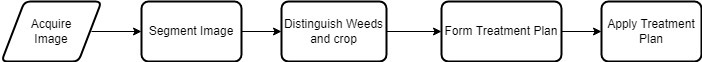
\includegraphics[width=0.75\linewidth]{./figures/image-processing-workflow.jpg}
	\caption{Image processing workflow}
	\label{fig:image-processing-workflow}
\end{figure}

 \newpage
 
\section{Objective and Aims}
The objective of this study is to not only answer the questions identified in the previous section, but to produce a viable system for field deployment. 

\subsection{Specific Aims}
The aims of this study will be to solve several problems in addition to the key questions posed earlier:
\begin{itemize}
	\item{Survey and develop image segmentation techniques that operate in the lighting conditions encountered in field conditions}
	\item{Develop machine learning approaches to discriminate between crop and weed that operate within the targeted time budget}
	\item{Design and integrate a system that will incorporate all aspects of the workflow shown in Figure~\ref{fig:image-processing-workflow}}
\end{itemize}
\newpage

%
% L I T E R A T U R E  R E V I E W 
%

\section{Background and Significance}

\subsection{Herbicide Exposure}
Exposure to synthetic herbicides \cite{Rydz2021-ar}
\subsection{Image Segmentation}
Humuda discusses  algorithms to separate the vegetated portion of an image from non-vegetated portions \cite{Hamuda2016-dw}. Specifically, this review compares the efficacy of approaches based on color index in visible light images. This paper details the formulae for various approaches. Hunt details an approach to segmentation that takes into account the responsiveness of the sensor \cite{Hunt2013-ih}.
{\renewcommand{\arraystretch}{2}%

% Example to span two pages
\begin{longtable}{x{\dimexpr.2\columnwidth-2\tabcolsep}
                  x{\dimexpr.4\columnwidth-2\tabcolsep}
                  x{\dimexpr.4\columnwidth-2\tabcolsep}}
%\begin{hyphenrules}{nohyphenation}
    \caption{Visible light indices}\label{tab:example}  \\
\toprule
{\textbf{Index}} & {\textbf{Formula}} & {\textbf{Comment}}
\tabularnewline
\midrule
    \endfirsthead
%%%%
    \caption{Visible light indices (cont.)}\label{tab:example}  \\
\toprule
{\textbf{Index}} & {\textbf{Formula}} & {\textbf{Comment}}
\tabularnewline
\midrule
    \endhead
%%%%
\midrule[\heavyrulewidth]
\multicolumn{3}{r}{\footnotesize\itshape
                   Continued on the next page}
    \endfoot
%%%%
\bottomrule
    \endlastfoot
%%%%
		Triangular Greenness
		& \begin{minipage}[t]{0.3\textwidth}
			$R_{green} - \alpha R_{red} - \beta R_{blue}\\ \alpha = \frac {2(\lambda_{blue} - \lambda_{green})} {(\lambda_{blue} - \lambda_{red})}\\ 
		    	\beta = \frac {2(\lambda_{green} - \lambda_{red})} {(\lambda_{blue} - \lambda_{red})} $
		   \end{minipage}     
		& Corrects for camera calibration using the peak sensitivity
\tabularnewline\addlinespace

		Normalized Difference     
		& $128 * \left( \left( \frac {(G - R)} {(G + R)} \right) + 1 \right) $                    
		& The NDI index produces a near-binary image. 
\tabularnewline\addlinespace

		Excess Green      
		& \begin{minipage}[t]{0.3\textwidth}
			$R = \frac {R} {R_{max}}\\ G = \frac {G} {G_{max}}\\ B = \frac {B} {B_{max}}$ 
		   \end{minipage}
		& ExG provided a clear contrast between plants and soil 
\tabularnewline\addlinespace

		Excess Red      
		& $1.3 R - G$ 
		& inspired by the fact that there are 4\% blue, and 32\% green, compared with 64\% red cones in the retina of the human eye
\tabularnewline\addlinespace

		Color Index of Vegetation Extraction      
		& $0.441 R - 0.811 G + 0.385 B + 18.78745$
		& This method was proposed to separate green plants from soil background in order to evaluate the crop growing status.
\tabularnewline\addlinespace

		Excess Green - Excess Red   
		& $ExG - ExR$ 
		& ExG used to extract the plant region and ExR used to eliminate the background noise (soil and residue) where green–red material (stems, branches, or petioles) may exist
\tabularnewline\addlinespace

		Normalized Green-Red Difference    
		& $\frac {(G - R)} {(G + R)}$ 
		& The method of NGRDI was used to overcome the differences in exposure settings selected by the digital camera when acquiring aerial photography of the field. 
\tabularnewline\addlinespace

		Vegetative Index      
		& $\frac {G} {R^aB^{(1-a)}}, a = 0.667$ 
		& VEG has a significant advantage because it is robust to lighting change.
\tabularnewline\addlinespace

		Com1   
		& $ExG + CIVE + ExGR + VEG$ 
		& TODO
\tabularnewline\addlinespace

		Modified Excess Green      
		& $1.262G - 0.884R = 0.311B$ 
		& TODO 
\tabularnewline\addlinespace

		Combined Indices 2      
		& $0.36ExG + 0.47CIVE + 0.17VEG$ 
		& Uses weighting factors to emphasize strengths of various approaches
\tabularnewline\addlinespace

\tabularnewline\addlinespace
\end{longtable}
% End example
Otsu describes an approach to automatically select thresholds in images \cite{Otsu1979-io}


%\end{longtable}
\subsection{Weed Identification}
In the proposed workflow, two sets of features are extracted from vegetation in the images: structural and color. Wirth gives an overview of the structural shape features used in this study: compactness, elongation, eccentricity, roundness, convexity and solidity \cite{Wirth2004-li}. 
Sabzi presents an analysis of factors for weed/crop discrimination that include both structural and color features \cite{Sabzi2020-af}. In that study, Sabzi identifies these features that produce a 98\% correct classification rate: saturation in the HSV \cite{Various_undated-yv} color space, the mean value of Hue in the HSI color space, the area to length ratio, the mean Chrominance component in the YCbCr \cite{Wikipedia_contributors2022-qd} color space, and the standard deviation of the in-phase component of the YIQ \cite{Various_undated-cz} color space.
Hemming studies using both morphological and color features, concluding that color features increase the accuracy of using morphological features alone. \cite{Hemming2001-ue} \\

Sabzi \cite{Sabzi2020-af} employs both color and morphological features in crop/weed discrimination:
\begin{itemize}
	\item{gray level co-occurrence matrix (GLCM)}
	\item{the standard deviation of saturation (S) component in HSV color space}
	\item{difference of first and seventh moment invariants}
	\item{mean value of hue component (H) in HSI color space} 
	\item{area to length ratio}
	\item{average blue-difference chrominance (Cb) component in YCbCr color space}
	\item{standard deviation of in-phase (I) component in YIQ color space}
\end{itemize}


\newpage
 
\section{System}
\label{section:system}

The system consists of three major subsystems: image processing, odometry, and treatment. Of these subsystems, only the image processing and odometry systems are covered in this study. The treatment sub-system has been developed separately \cite{Siemens2020-ds}, and will not be explored in-depth in this proposal. While treatment is important to the overall efficacy of the system, the realization of the treatment through mechanics, chemical, or other means (lasers) will not have significant bearing on this proposal. The image processing system uses machine learning to distinguish weed from crop and will direct treatment of vegetation deemed to be a weed, and represents the bulk of this proposal. 

The system will be realized as an integrated solution, towed behind a tractor, treating a single bed with two crop rows as it travels along the row.
\begin{figure}[H]
	\centering
	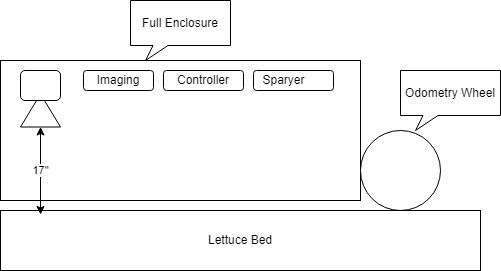
\includegraphics[width=0.4\linewidth]{./figures/system-in-field.jpg}
	\caption{The system in the field}
	\label{fig:system-in-field}
\end{figure}

The integrated system is composed of four components:
\begin{itemize}
\item{A machine-vision camera, contained in a protective housing, and mounted on a gimbal system}
\item{An image processing system, where weeds within the images acquired by the camera and treatment plans formed}
\item{A controller, whose duties are to interpret signals from the odometry system and to direct the treatment/sprayer subsystem}
\item{A treatment subsystem, here, a high-precision sprayer}
\end{itemize}

Figure~\ref{fig:system-overview} illustrates how the system will be realized for a single-bed, two-row system. In this realization, some components are dedicated to a crop row (the camera and associated lighting) and some are shared as a central resource (the National Instruments RIO controller)
\begin{figure}[H]
	\centering
	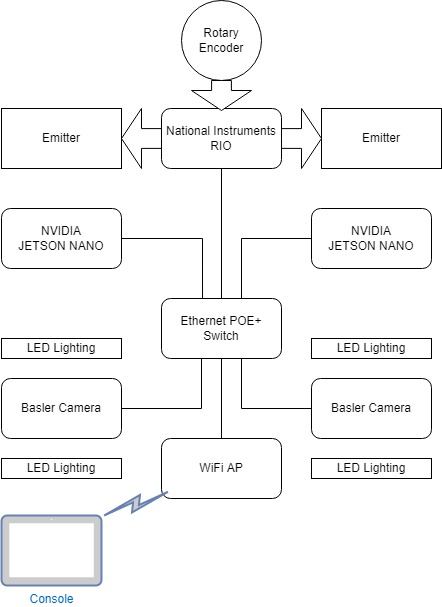
\includegraphics[width=0.4\linewidth]{./figures/system-overview.jpg}
	\caption{An overview of the system}
	\label{fig:system-overview}
\end{figure}
\subsection{Development Environment and Software Components}
The software development environment will consist of:
\begin{itemize}
	\item{Microsoft Windows 10}
	\item{PyCharm Python IDE version 2020.3}
\end{itemize}
All software will be developed using Python 3.8 with these software and hardware components:
\begin{itemize}
	\item{Prosody XMPP Server}
	\item{Slix XMPP Client Library}
	\item{Scikit-Learn}
	\item{NumPy}
	\item{National Instruments daqmx Python Library}
	\item{Basler Pylon Python Library}
	\item{NVIDIA Jetson Nano}
	\item{National Instruments CompactRIO}
\end{itemize}

\subsection{Component Communication} 
In this system, components communicate with each other through a publish-and-subscribe technique using Extensible Messaging and Presence Protocol (XMPP). This technique has been likened to a chat-room, and for the purposes here, that analogy will suffice. In such a system, components simply announce findings, and whoever is interested in receiving those messages will do so and will possibly respond. This technique lends itself to a \textit{loosely coupled} system, one in which the composition of the system can be quite easily altered\footnote{While not a direct goal of the work outlined here, this arrangement simplifies making the system components redundant and the entire system fault tolerant} Consider the arrangement where the processing of an image is carried out by one of a dozen processing subsystems. Inserting new processing components into a loosely coupled system is trivial.
In Figure~\ref{fig:system-overview}, there are three different connections: Ethernet, Serial, and WiFi. Serial cables are used to provide point-to-point connections between the controller and the encoder and the emitters. The Ethernet and WiFi networks host the XMPP traffic the networked components use for communication. There are three chatrooms (or channels) in this system:
\begin{itemize}
	\item{Distance}
	\item{Treatment}
	\item{Administration}
\end{itemize}
The Odometry subsystem, for instance, may not be concerned at all with treatment computations, and does not subscribe to that communications channel. An important aspect of this communication is that interested parties receive messages simultaneously, and for the purposes of this system, this is key. The correct functioning of both the treatment and image processing systems are dependent on distance, and simultaneous delivery avoids much of the adjustments that would be required in messages were delivered in series.

\subsection{Machine Vision - Basler Camera}
The machine vision system hosts no software written as part of this project.  Its sole function is to continuously stream a set of images to the image processing subsystem\cite{noauthor_undated-tt}.  The acquisition of images in ambient light (daylight) is full of challenges, the most prominent of which is dealing with varying lighting conditions due to obstructions, cloud-cover, and time-of-day. In this system, images are acquired with all illumination supplied by LED lighting under controlled conditions. All external illumination (natural light from the sun and stray artificial light) is blocked by the housing of the system itself. In this system images are acquired continuously, but \textit{selected} from that stream only when the system has moved into the correct position.

\subsection{Odometry - Rotary Encoder}
The odometry subsystem consists of an incremental encoder used to detect changes in wheel position and the software that makes that determination and announces its findings to the rest of the system. The odometry subsystem software resides within the controller, interpreting signals it receives from the directly attached rotary encoder. As the system moves forward, the odometry system makes announcements of distance traveled that are in line with the precision of the treatment subsystem. 

\subsection{Image Processing - NVIDIA Jetson}
The image processing subsystem is hosted on an NVIDIA Jetson Nano platform, a standalone GPU, and has three responsibilities:
\begin{enumerate}
\item{Acquire images from a stream of images issued by the machine vision camera when the system has moved forward a specific distance}
\item{Identify weeds in an acquired image}
\item{Form and announce a treatment plan}
\end{enumerate} 

This deployment platform is geared toward optimizing machine learning problems without the overhead of a CPU-based system hosting a GPU.
 
\subsection{Console}
The console is the mechanism for an operator to interact with the system. Figure~\ref{fig:console-operator} illustrates a concept that allows an operator to:
\begin{itemize}
	\item{See the treatment plan currently being applied}
	\item{See the current state of each sprayer}
	\item{See overall statistics for a weeding session}
	\item{Control weeded operations, starting and stopping as required}
\end{itemize}
	

\begin{figure}[H]
	\centering
	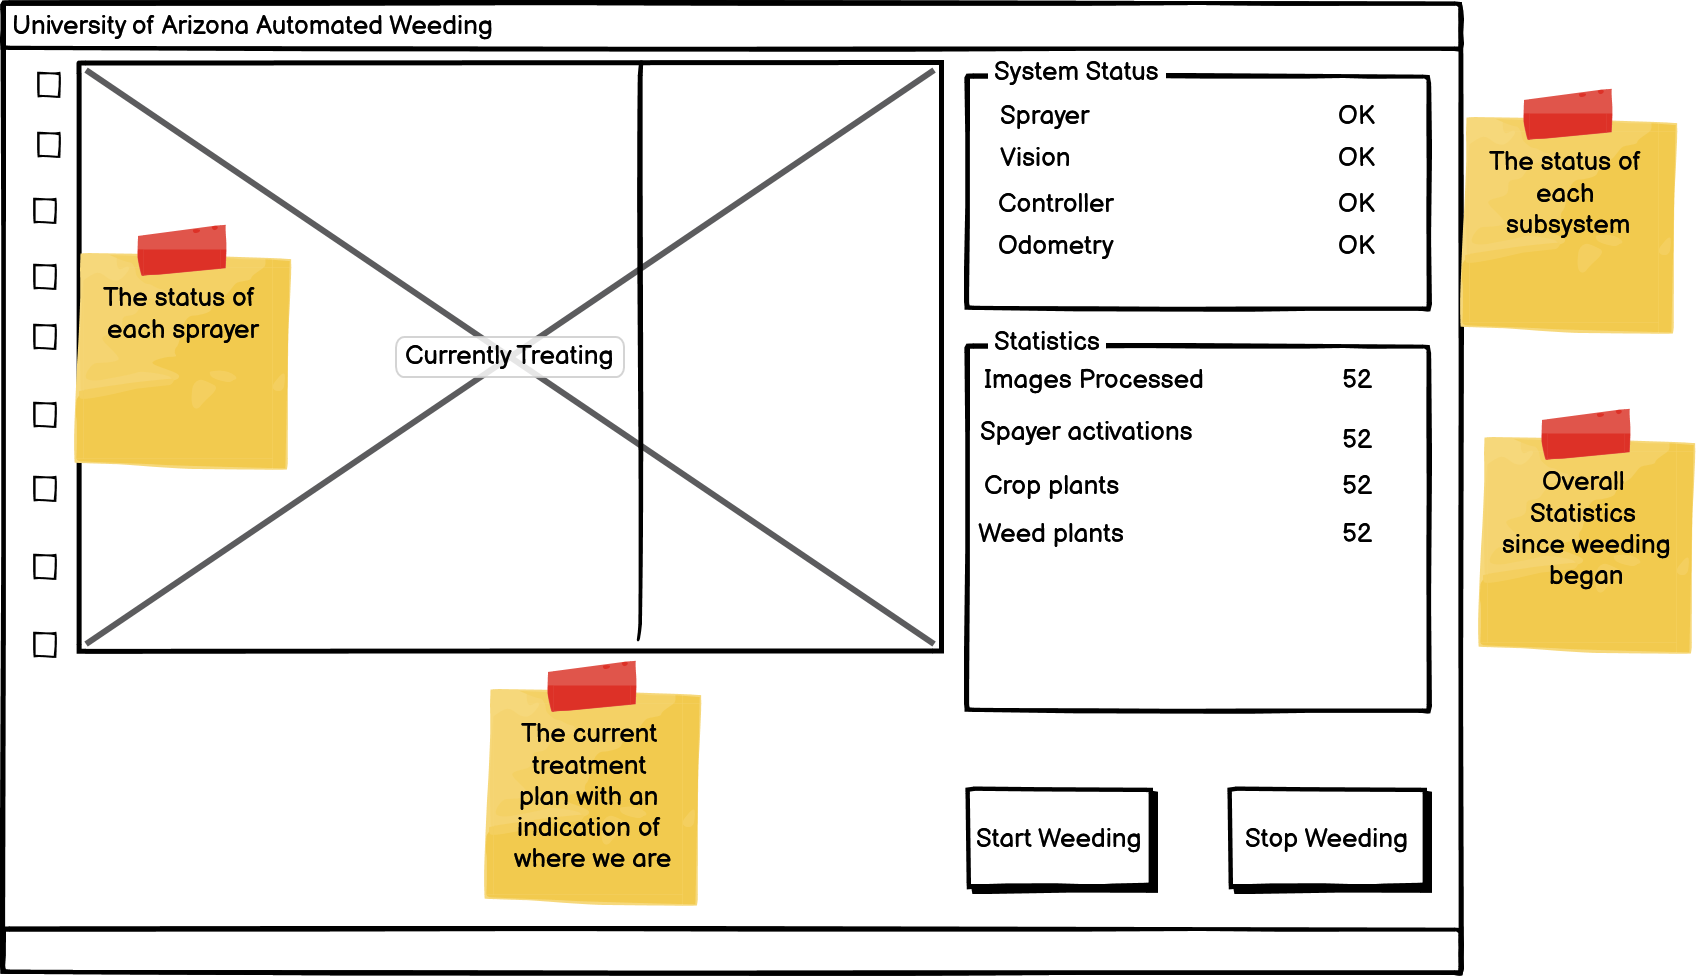
\includegraphics[width=0.75\linewidth]{./figures/console-operator.png}
	\caption[An operator's console]{An operator's console that presents an overview of the current system state}
	\label{fig:console-operator}
\end{figure}

While it is unlikely that the final console will take on this exact form, a few guiding principles will guide the final design of this:
\begin{itemize}
	\item{The interface will have as few large controls as possible, for instance large, easily accessed buttons}
	\item{The interface will be internationalized (I18N), with Spanish and English interfaces the first two languages developed}
	\item{The interface will be optimized for use on mobile devices}
\end{itemize}

Once again, we see an advantage of using a publish-subscribe mechanism of communication. The rest of the system has no knowledge that there is an operator's console, and can be developed without factoring that knowledge that it even exists. That is, the treatment system does not tell the console that sprayer \#4 has been activated, it simply announces that it has activated that sprayer.  The console reports the events it observes in the chatrooms.

\subsection{Phasing}
This work will be carried out in three phases:
\begin{itemize}
\item{Proof of concept: In this phase some fundamental questions are answered, such as \textit{can weeds and crops be distinguished using visible light images?}}.
\item{Prototype: This phase concentrates on using physical hardware targeted for field use: a camera, an NVIDIA GPU, and a National Instruments Controller. A key question answered in this phase is \textit{can images be processed fast enough to support a commercially viable speed?}}
\item{Production: This phases shifts the focus to the field, where the physical hardware integrated in the previous phase brought together with the existing mechanicals and is proven under real-world conditions.} 
\end{itemize}

\subsubsection{Proof of concept}
This phase will explore and develop the basic approaches to image segmentation and crop/weed discrimination. The target images for this phase will come in two forms: image sets that have been collected in the field, and composed images where various weed placements are tested.
\subsubsection{Prototype}
This phase will integrate software with hardware that will be used in the field, and will integrate with the XMPP communications channel that will be used in the field. The prototype phase will encompass these activities: \\
\begin{itemize}
	\item{Complete the image recognition, odometry, and treatment solution subsystems}
	\item{Integrate with the Basler machine vision camera}
	\item{Port the image processing system to the NVIDIA Jetson and integrate with the hosted GPU}
	\item{Port the odometry system to the National Instruments RIO}
	\item{Port the treatment system to the National Instruments RIO}
	\item{Integrate component communication}
\end{itemize}
\subsubsection{Production}
This phase will have two activities: installation of the physical hardware in the field enclosure, and field testing of the system. This phase will encompass these activities:
\begin{itemize}
	\item{Modify the existing enclosure and install components discussed in Section~\ref{section:system}}
	\item{Field test the integrated system}
\end{itemize}

 \newpage
%
% W E A K N E S S E S
%
\section{Weaknesses of Study}
This proposal has weaknesses in two areas: weed/crop discrimination under field conditions and system redundancy.

\subsection{Weed/Crop discrimination}
While the concepts around this are explored in the proof of concept phase, the image sets used there are obtained under lighting conditions that will  not be encountered in the production phase. The structural features noted previously will probably be invariant to changes based on lighting -- how round an object is does not depend heavily on lighting conditions, for instance. Color features, however, may. Vegetation may exhibit different responses to LED light than to full-spectrum sunlight.

\subsection{Redundancy}
The system described in this proposal has multiple single points of failure. In such a system, for instance, the failure of a shared resource -- such as the National Instruments RIO controller -- would render the entire system unusable. The failure of a resource dedicated to a task, but with a peer performing the same task -- such as processing the images along the right side of a row -- will result in the degradation of system, but not a complete failure.
\begin{figure}[H]
	\centering
	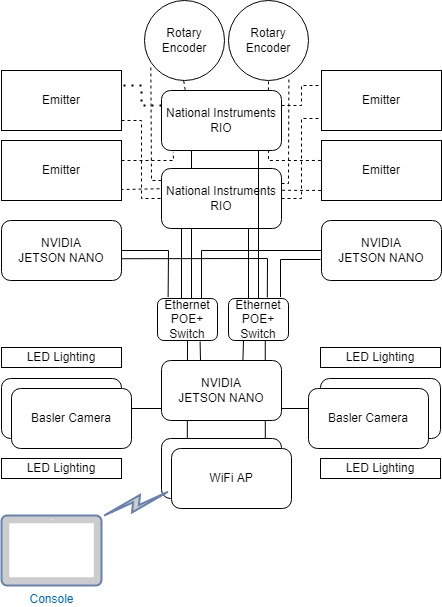
\includegraphics[width=0.4\linewidth]{./figures/system-overview-Page-2.jpg}
	\caption[An overview of a redundant system]{An overview of a redundant system, illustrating that there is no single point of failure}
	\label{fig:system-overview-redundant}
\end{figure}

Figure~\ref{fig:system-overview-redundant} illustrates a system without a single point of failure. If a RIO controller fails, for example, the system can use the redundant controller. If an Ethernet switch fails or if a cable fails connecting a component, that component can use the redundant network. In these systems, there are redundancy decisions that can be made locally -- a link to a switch has failed and the other switch must be used --- and redundancy decisions that must be made system-wide -- the failure of a component hosting the messaging server, for instance. That the system shows three NVIDIA devices is indicative of the N+1 redundancy scheme used by such a system. This system can tolerate the loss of only one NVIDIA, as it must have a \textit{quorum} of members to form a redundancy group. It is beyond the scope of this proposal to discuss redundancy schemes in depth, and the overly broad statements here are not meant to be an analysis of failure scenarios.
 
%\newpage
%\section{Public Health Significance}
 
\section{Budget}
\label{section:budget}
Table~\ref{table:budget} reflects the total expenditures involved in this study. While not broken down by year, it is anticipated that these expenditures will take place over two years. Amounts specified are in US\$.
\begin{table}[h]
\centering
\begin{tabular}{lrlr}
 	\toprule
	Salaries/Wages    &  & 2670.60 \\
	\midrule
	& Mechanicals & 1965.00 \\
	&Field Operator & 705.60 \\
	\midrule
	Travel & & 2241.72 \\
	\midrule
	& In State & 2241.72 \\
	\midrule
	Supplies & & 6789.00 \\
	\midrule
	\midrule
	Project subtotal & & 11701.32 \\
	\midrule
	Indirect Costs (53\%)\tablefootnote{This may not be required if separate funding is not obtained. If that is not the case, the project subtotal should be considered the grand total for the project.} & & 6201.70 \\
	\toprule
	\toprule
	\textsc{Total Project}                      & & \underline{18387.92} \\

	\bottomrule
    \bottomrule                
\end{tabular}
\caption[Total Budget Breakdown]{A breakdown of expenditures for this study}
\label{table:budget}
\end{table}

%
% S A L A R I E S
%
\subsection{Salaries and Wages}
Table~\ref{table:salaries} reflects the salary expenditures for this study.  The components discussed in Section~\ref{section:system} will need to be installed in the existing enclosure. To accommodate these components, mechanical modifications will be required and will be carried out at the Yuma Agricultural Research Center. Once a modified system is ready, an operator qualified to operate a tractor in a field setting will conduct test runs using the system at the Valley Farm site of the Yuma Agricultural Research center.
\begin{table}[H] % Force the table to show below the paragraph
\centering
\begin{tabular}{lrlrlrlrlrlrlr}
 	\toprule
	Role & Per Hour & Hours Per Week & Weeks & ERE & Subtotal \\
	\toprule
	Mechanicals & 25.00 & 20 & 3 & 31.0\% & 1965.00 \\
	Field Operator & 15.00 & 2 & 20 & 17.6\% & 705.60 \\
	\toprule
	\toprule
	\textsc{Total Salaries} & & & & & \underline{2670.60} \\

	\bottomrule
    \bottomrule                
\end{tabular}
\caption[Salary Breakdown]{A breakdown of salaries for this study}
\label{table:salaries}
\end{table}

%
% T R A V E L
%

\subsection{Travel}
Travel funds dedicated for in-state travel represent 6 trips to Yuma, Arizona to oversee physical system integration of the automated system and to oversee and collect data from field trials. These activities both take place at the University of Arizona Yuma Agricultural Center.
\begin{table}[H] % Force the table to show below the paragraph
\centering
\begin{tabular}{lrlr}
 	\toprule
	\toprule
	6 Trips to Yuma, AZ & & 2241.72 \\
	\midrule
	& Vehicle Rental for 2 days per trip @ \$67.31 & 1407.72 \\
	& Lodging for 1 day per trip @ \$94.00 & 564.00 \\
	& M\&IE for 2 days per trip @ \$45.00 & 270.00 \\
	\toprule
	\toprule
	\textsc{Total Travel}                      & & \underline{2241.72} \\
	\bottomrule
    \bottomrule                
\end{tabular}
\caption[Travel Budget Breakdown]{A breakdown of travel expenditures for this study}
\label{table:travel}
\end{table}

%
% S U P P L I E S
%
\subsection{Supplies}
Table~\ref{table:supplies} reflects the supply expenditures for this proposal. All of the supplies here represent the Bill of Materials (BOM) of the final system, and will be installed in the existing enclosure. These supplies are required to support the completion of the \textit{deployment} phase detailed in Section~\ref{section:phases}.\\

\begin{table}[H] % Force the table to show below the paragraph
\centering
\begin{tabular}{lrlr}
 	\toprule
 	Item & Quantity & Price \\
 	\midrule
	Heavy Duty TRD-GK Rotary Encoder & 1 & 269.00 \\
	NVIDIA Jetson & 2 @ 459 &918.00 \\
	NVIDIA Jetson Enclosure &2 @ 25 & 50.00 \\
	LED Lamps & 4 @ 150 & 600.00 \\
	National Instruments CompactRIO&1& 1567.00 \\
	9411 Module for RIO &1& 372.00 \\
	9403 Module for RIO &1& 656.00 \\
	Cables &6+& 75.00 \\
	Basler ACE2 Machine Vision Camera &2 @ 730& 1460.00  \\
	Computar C-Mount Lens &2 @ 320& 640.00 \\
	POE+ Ethernet Switch &1& 50.00 \\
	WiFi Outdoor Access Point &1& 70.00 \\
	Encoder Power Supply &1& 12.00 \\
	NVIDIA Jetson Power Supply &2 @ 25& 50.00 \\
	\midrule
	\midrule
	\textsc{Total Supplies}                      & & \underline{6789.00} \\
	\bottomrule
    \bottomrule                
\end{tabular}
\caption[Supply Budget Breakdown]{A breakdown of supply expenditures for the deployment stage of this study}
\label{table:supplies}
\end{table}




%\end{table}

%REFERENCES
%Use the Vancouver Style of referencing. This is found at this website:
%http://www.ncbi.nlm.nih.gov/books/bv.fcgi?rid=citmed.TOC&depth=2 or a less detailed website:
%http://www.nlm.nih.gov/bsd/uniform_requirements.html
%
%References should be numbered consecutively in the order in which they are first mentioned in the text. Identify references in text, tables, and legends by Arabic numerals in parentheses. The titles of journals should be abbreviated according to the style used in Index Medicus. Consult the list of Journals Indexed for MEDLINE, published annually as a separate publication by the National Library of Medicine. The list can also be obtained through the Library's web site..



 


% 
% E N D  T E M P L A T E  F R O M  W O R D
%

\newpage
\section{References}
\printbibliography[heading=none]

%\cite{Wirth2004-li}
\end{document}

